% documentclass, begin, end comprise the basic layout of a LaTeX file
% LaTeX command syntax is \commandname{option}
% \begin & \end define `environments' areas of a document where certain typesetting rules apply
% sort of like CSS, it is imperative the `document' environment is topmost, however.
% LaTeX comes with predefined environments, you can define your own, but it likely exists.

\documentclass{article}

% this is a package import
% packages must be declared in the preamble.
\usepackage{amsmath}
\usepackage{graphicx}
\usepackage{float}
\usepackage{subcaption}

% extra commands to setup title page
% this area before our main document is called the `preamble'
\title{Learning \LaTeX{} by doing.}
\date{\today}
\author{Dig03}

% you can also define sections within a document (for paragraphing and the like)
% they are: section, subsection, subsubsection, ..., paragraph, subparagraph
\begin{document}

\pagenumbering{gobble} % set preference to ignore page numbers
\maketitle % title page
\newpage   % page break
\pagenumbering{arabic} % turn page numbers back on, `roman' for roman numbering

\section{General Initial Thoughts}

Hello, world!

\subsection{Even More Specific Thoughts}

Sometimes, I dream about cheese.

\subsubsection{Unreasonably Specific Thoughts}

I think we've gone too deep.

\paragraph{A Paragraph}

This is a paragraph.

\subparagraph{A Subparagraph}

This is a subparagraph.

\section{Surprise Section}

\section{Math environment features}

\subsection{equation}

\begin{equation}
	f(x) = x^2
\end{equation}

\subsection{equation*}

This environment is provided by the package `amsmath', and removes automatic numbering.

\begin{equation*}
	f(x, y) = x^2 + y^2 + c
\end{equation*}

\subsection{align*}

This environment is needed for aligning multiple equations.

\begin{align*}
	1 + 2 &= 3\\
	1 &= 3 - 2
\end{align*}

Here we see that the equations are aligned such that the equalities are lined up.
Equations are aligned at the ampersand (\&). Equations are separated with linebreaks (\textbackslash\textbackslash).

\subsection{Fractions and more}

\begin{align*}
	f(x) &= x^2\\
	g(x) &= \frac{1}{x}\\
	F(x) &= \int^a_b \frac{1}{3}x^3
\end{align*}

`int' here for integrals, and `frac' for fractions.

`sqrt' also exists, and can be nested like so:

\begin{equation*}
	\frac{1}{\sqrt{x}}
\end{equation*}

More complicated expressions naturally become more error prone. Therefore you should take great care in opening and closing the braces (\{\}). Much time may be wasted on debugging such errors. The \textit{Lyx} program offers a great formula editor, which can ease this.

\subsection{Matrices}

\begin{equation*}
	\begin{matrix}
		1 & 0\\
		0 & 1
	\end{matrix}
\end{equation*}

Must be defined within a math environment (equation, equation*, align*, inline).

To surround the matrix by brackets we must use special statements. This ensures scaling works properly.

\begin{equation*}
	\left[
	\begin{matrix}
		1 & 0\\
		0 & 1
	\end{matrix}
	\right]
\end{equation*}

This also works for parentheses and braces and is not limited to matrices:

\begin{equation*}
	\left(\frac{1}{\sqrt{x}}\right)
\end{equation*}

\section{Math Features (non-environment)}

\subsection{Inline math}
The following is an example of inline math: $f(x) = x^2$.

\section{Figures and Images}

The following requires the `graphicx' package.

\subsection{Figure environment}

\begin{figure}[H]
	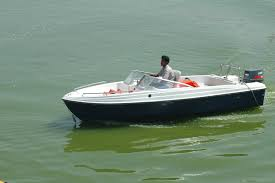
\includegraphics[width=\linewidth]{boat.jpg}
	\caption{A boat.}
	\label{fig:boat1}
\end{figure}

Figure \ref{fig:boat1} shows a boat.

The `float' can be set on figures. It consists of a couple possible values.
h (here), t (top), b (bottom), p ([extra] page), ! (override), H (float package, stricter h!).

\subsection{Subfigure environment}

Usually you won't be adding single images, you'll want multiple to aid comparison.
For this, you'll need a different environment called subfigure, provided by `subcaption'.

\begin{figure}[h!]
  \centering
  % rule, width should be .1 smaller than expected
  % e.g. 1/2 - 0.5 -> ( - .1 ) -> 0.4
  \begin{subfigure}[b]{0.4\linewidth}
    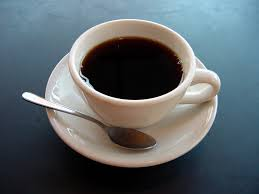
\includegraphics[width=\linewidth]{coffee.jpg}
    \caption{Coffee.}
  \end{subfigure}
  \begin{subfigure}[b]{0.4\linewidth}
    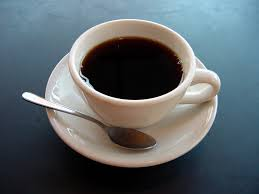
\includegraphics[width=\linewidth]{coffee.jpg}
    \caption{More coffee.}
  \end{subfigure}
  \caption{The same cup of coffee. Two times.}
  \label{fig:coffee}
\end{figure}

\begin{figure}[h!]
  \centering
  \begin{subfigure}[b]{0.2\linewidth}
    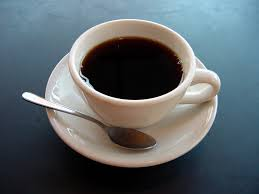
\includegraphics[width=\linewidth]{coffee.jpg}
     \caption{Coffee.}
  \end{subfigure}
  \begin{subfigure}[b]{0.2\linewidth}
    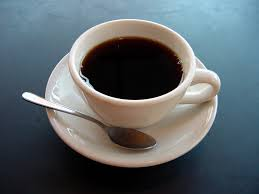
\includegraphics[width=\linewidth]{coffee.jpg}
    \caption{More coffee.}
  \end{subfigure}
  \begin{subfigure}[b]{0.2\linewidth}
    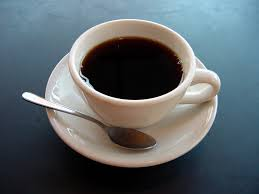
\includegraphics[width=\linewidth]{coffee.jpg}
    \caption{Tasty coffee.}
  \end{subfigure}
  \begin{subfigure}[b]{0.5\linewidth}
    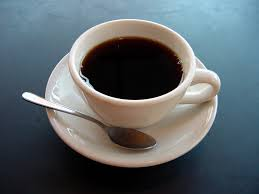
\includegraphics[width=\linewidth]{coffee.jpg}
    \caption{Too much coffee.}
  \end{subfigure}
  \caption{The same cup of coffee. Multiple times.}
  \label{fig:coffee3}
\end{figure}

\end{document}

% BOOKMARK: 06 Table of contents https://www.latex-tutorial.com/tutorials/table-of-contents/